\documentclass[12pt]{standalone}
\usepackage{tikz, pgfmath}
\usetikzlibrary{calc, decorations.pathreplacing}


% draw stack of mapped reads
%
% Parameters
% #1: SNP coordinate on reference genome
% #2: number of reads
% #3: + or - depending on the direction to grow the stack (up or down, respectively)
% #3: + or - depending on small baseline correction to avoid reads overlap at neighboring SNPs (up or down, respectively)
% #5: style of the read
% #6: style of the SNP variant on the read
\newcommand{\mappedreads}[6]{
\path #1 ++(0, #3 5pt) ++(0, #4 0.75pt) coordinate (baseline);
\draw[#5] let \n1 = {0.2} in foreach \y in {1,...,#2} { (baseline) ++(0, \y * #3 3pt) node[#6] {} ++(rand * \n1, 0) +(-\n1,0) -- +(\n1,0) };
}


% draw DNA molecule with all SNP variants
%
% Parameters
% #1: style of DNA
% #2: a coordinate to determine vertical position
% #3-6: style of SNP variants
\newcommand{\DNAgenomeone}[6]{
\coordinate (horiz) at #2;
\path (horiz) ++(0,3pt) coordinate (geneupperedge);
\path[orf] (g1g1start|-horiz) ++(0,-3pt) rectangle (g1g1end|-geneupperedge);
\path[orf] (g1g2start|-horiz) ++(0,-3pt) rectangle (g1g2end|-geneupperedge);
\draw[#1] (g1start|-horiz) -- (g1g1s1|-horiz) node[#3] {} -- (g1g1s2|-horiz) node[#4] {} -- (g1g1s3|-horiz) node[#5] {} -- (g1g2s1|-horiz) node[#6] {} -- (g1end|-horiz);
}

% a horizontally shifted version of \DNAgenomeone
\newcommand{\DNAgenometwo}[6]{
\coordinate (horiz) at #2;
\path (horiz) ++(0,3pt) coordinate (geneupperedge);
\path[orf] (g2g1start|-horiz) ++(0,-3pt) rectangle (g2g1end|-geneupperedge);
\path[orf] (g2g2start|-horiz) ++(0,-3pt) rectangle (g2g2end|-geneupperedge);
\draw[#1] (g2start|-horiz) -- (g2g1s1|-horiz) node[#3] {} -- (g2g1s2|-horiz) node[#4] {} -- (g2g1s3|-horiz) node[#5] {} -- (g2g2s1|-horiz) node[#6] {} -- (g2end|-horiz);
}


% draw DNA molecule with all SNP variants
%
% Parameters
% #1: style of DNA
% #2: a coordinate to determine vertical position
\newcommand{\matRNAgenomeone}[7]{
\foreach \y in {1,...,#6} {
\path #1 +(0, \y * 3pt) coordinate (hrz);
\draw[matread]
(g1g1start|-hrz) -- (g1g1s1|-hrz) node[#2] {} -- (g1g1s2|-hrz) node[#3] {} -- (g1g1s3|-hrz) node[#4] {} -- (g1g1end|-hrz);
}
\foreach \y in {1,...,#7} {
\path #1 +(0, \y * 3pt) coordinate (hrz);
\draw[matread]
(g1g2start|-hrz) -- (g1g2s1|-hrz) node[#5] {} -- (g1g2end|-hrz);
}
}

% the paternal version of \matRNAgenomeone
\newcommand{\patRNAgenomeone}[7]{
\foreach \y in {1,...,#6} {
\path #1 +(0, -\y * 3pt) coordinate (hrz);
\draw[patread]
(g1g1start|-hrz) -- (g1g1s1|-hrz) node[#2] {} -- (g1g1s2|-hrz) node[#3] {} -- (g1g1s3|-hrz) node[#4] {} -- (g1g1end|-hrz);
}
\foreach \y in {1,...,#7} {
\path #1 +(0, -\y * 3pt) coordinate (hrz);
\draw[patread]
(g1g2start|-hrz) -- (g1g2s1|-hrz) node[#5] {} -- (g1g2end|-hrz);
}
}

% a horzontally shifted version of \matRNAgenomeone
\newcommand{\matRNAgenometwo}[7]{
\foreach \y in {1,...,#6} {
\path #1 +(0, \y * 3pt) coordinate (hrz);
\draw[matread]
(g2g1start|-hrz) -- (g2g1s1|-hrz) node[#2] {} -- (g2g1s2|-hrz) node[#3] {} -- (g2g1s3|-hrz) node[#4] {} -- (g2g1end|-hrz);
}
\foreach \y in {1,...,#7} {
\path #1 +(0, \y * 3pt) coordinate (hrz);
\draw[matread]
(g2g2start|-hrz) -- (g2g2s1|-hrz) node[#5] {} -- (g2g2end|-hrz);
}
}

% the paternal version of \matRNAgenometwo
\newcommand{\patRNAgenometwo}[7]{
\foreach \y in {1,...,#6} {
\path #1 +(0, -\y * 3pt) coordinate (hrz);
\draw[patread]
(g2g1start|-hrz) -- (g2g1s1|-hrz) node[#2] {} -- (g2g1s2|-hrz) node[#3] {} -- (g2g1s3|-hrz) node[#4] {} -- (g2g1end|-hrz);
}
\foreach \y in {1,...,#7} {
\path #1 +(0, -\y * 3pt) coordinate (hrz);
\draw[patread]
(g2g2start|-hrz) -- (g2g2s1|-hrz) node[#5] {} -- (g2g2end|-hrz);
}
}


\newlength{\m} % 1 meter
\setlength{\m}{25pt}

\tikzset{ man/.pic={ \node[human] {\includegraphics[height=1.7\m]{/home/attila/figures/stock-images/man-in-hat.jpg}}; } }
\tikzset{ gray-man/.pic={ \node[human] {\includegraphics[height=1.7\m]{/home/attila/figures/stock-images/man-in-hat-gray.jpg}}; } }
\tikzset{ man-old/.pic={ \node[human] {\includegraphics[height=1.5\m]{/home/attila/figures/stock-images/man-old.jpg}}; } }
\tikzset{ gray-man-old/.pic={ \node[human] {\includegraphics[height=1.5\m]{/home/attila/figures/stock-images/man-old-gray.jpg}}; } }
\tikzset{ woman-old/.pic={ \node[human] {\includegraphics[height=1.5\m]{/home/attila/figures/stock-images/woman-old.jpg}}; } }
\tikzset{ gray-woman-old/.pic={ \node[human] {\includegraphics[height=1.5\m]{/home/attila/figures/stock-images/woman-old-gray.jpg}}; } }
\tikzset{ woman-a/.pic={ \node[human] {\includegraphics[height=1.6\m]{/home/attila/figures/stock-images/woman-hair-in-bun.jpg}}; } }
\tikzset{ gray-woman-a/.pic={ \node[human] {\includegraphics[height=1.6\m]{/home/attila/figures/stock-images/woman-hair-in-bun-gray.jpg}}; } }
\tikzset{ woman-b/.pic={ \node[human] {\includegraphics[height=1.6\m]{/home/attila/figures/stock-images/woman-hair-hanging.jpg}}; } }
\tikzset{ gray-woman-b/.pic={ \node[human] {\includegraphics[height=1.6\m]{/home/attila/figures/stock-images/woman-hair-hanging-gray.jpg}}; } }

\begin{document}
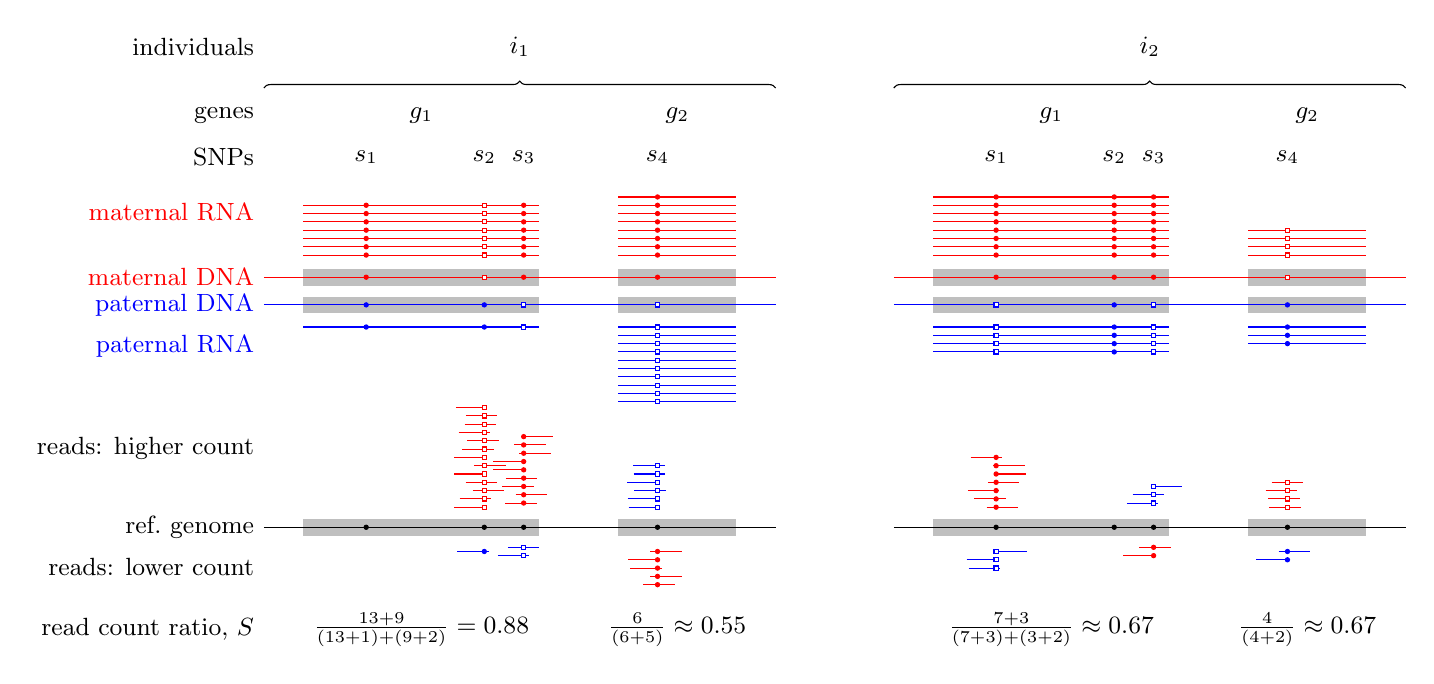
\begin{tikzpicture}[
% SNP variants
var/.style={minimum width=1.5pt, minimum height=1.5pt, inner sep=0, thin, rectangle},
alt/.style={var, draw, fill=white},
ref/.style={var, draw, fill, circle},
% RNA or DNA molecules
DNA/.style={},
matDNA/.style={DNA, red},
patDNA/.style={DNA, blue},
% RNA-seq reads
read/.style={},
matread/.style={read, red},
patread/.style={read, blue},
% genes (ORFs)
orf/.style={fill=lightgray, very thin},
% annotations
annot/.style={font=\small},
sideannot/.style={annot, anchor=east},
sideannotL/.style={sideannot, font=\large},
topannot/.style={annot, anchor=center},
% human silhouettes
human/.style={anchor=south}
]

\pgfmathsetseed{1976}

% HORIZONTAL COORDINATES

% genome1
\coordinate (g1start) at (0.5,0); % genome 1 start
\coordinate (g1g1start) at (1,0); % genome 1, gene 1 and its SNPs
\coordinate (g1g1s1) at (1.8,0);
\coordinate (g1g1s2) at (3.3,0);
\coordinate (g1g1s3) at (3.8,0);
\coordinate (g1g1end) at (4,0);
\coordinate (g1g2start) at (5,0); % genome 1, gene 2 and its SNPs
\coordinate (g1g2s1) at (5.5,0);
\coordinate (g1g2end) at (6.5,0);
\coordinate (g1end) at (7,0); % genome 1 end

% genome2
\path let \n1 = {8} in
(g1start) +(\n1,0) coordinate (g2start)
(g1g1start) +(\n1,0) coordinate (g2g1start)
(g1g1s1) +(\n1,0) coordinate (g2g1s1)
(g1g1s2) +(\n1,0) coordinate (g2g1s2)
(g1g1s3) +(\n1,0) coordinate (g2g1s3)
(g1g1end) +(\n1,0) coordinate (g2g1end)
(g1g2start) +(\n1,0) coordinate (g2g2start)
(g1g2s1) +(\n1,0) coordinate (g2g2s1)
(g1g2end) +(\n1,0) coordinate (g2g2end)
(g1end) +(\n1,0) coordinate (g2end)
;


% VERTICAL COORDINATES

\path[]
% RNA-seq
(0.5,1) node[sideannot] (RNAseq) {ref.~genome}
+(0,1) node[sideannot, align=center] {reads: higher count}
+(0,-0.5) node[sideannot, align=center] {reads: lower count}
% expression
++(0,3) node (expr) {}
+(0,1) node[sideannot, color=red] {maternal RNA}
++(0,5pt) node[sideannot, color=red] (matDNA) {maternal DNA}
+(0,5pt) node (matRNA) {}
(expr)
++(0,-5pt) node[sideannot, color=blue] (patDNA) {paternal DNA}
+(0,-5pt) node (patRNA) {}
+(0,-15pt) node[sideannot, color=blue] {paternal RNA}
% annotation of genes and SNPs above expression
(expr)
++(0,1.7) node[sideannot] (SNPs) {SNPs}
++(0,15pt) node[sideannot] (genes) {genes}
++(0,10pt) node[sideannot] (indiv) {}
+(0,15pt) node[sideannot] {individuals}
% read count ratio
(0.5,-0.3) node[sideannot] (S) {read count ratio, \(S\)}
;


% DRAW GENOME 1
% molecules/seqmences
\DNAgenomeone{matDNA}{(matDNA)}{ref}{alt}{ref}{ref}
\DNAgenomeone{patDNA}{(patDNA)}{ref}{ref}{alt}{alt}
\matRNAgenomeone{(matRNA)}{ref}{alt}{ref}{ref}{7}{8}
\patRNAgenomeone{(patRNA)}{ref}{ref}{alt}{alt}{1}{10}
\DNAgenomeone{DNA}{(RNAseq)}{ref}{ref}{ref}{ref}
\mappedreads{(g1g1s2|-RNAseq)}{13}{+}{-}{matread}{alt}
\mappedreads{(g1g1s2|-RNAseq)}{1}{-}{-}{patread}{ref}
\mappedreads{(g1g1s3|-RNAseq)}{9}{+}{+}{matread}{ref}
\mappedreads{(g1g1s3|-RNAseq)}{2}{-}{+}{patread}{alt}
\mappedreads{(g1g2s1|-RNAseq)}{6}{+}{-}{patread}{alt}
\mappedreads{(g1g2s1|-RNAseq)}{5}{-}{-}{matread}{ref}
% annotations
\path[decorate, decoration=brace, draw]
(g1start|-indiv) -- coordinate (i1) pic[anchor=south] {} (g1end|-indiv)
(i1) +(0pt,15pt) node[annot] {\(i_1\)}
;
\path
(g1g1start|-genes) -- node[topannot] {\(g_1\)} (g1g1end|-genes)
(g1g2start|-genes) -- node[topannot] {\(g_2\)} (g1g2end|-genes)
;
\path
(g1g1s1|-SNPs) node[topannot] {\(s_1\)}
(g1g1s2|-SNPs) node[topannot] {\(s_2\)}
(g1g1s3|-SNPs) node[topannot] {\(s_3\)}
(g1g2s1|-SNPs) node[topannot] {\(s_4\)}
;
% cohort of individuals
%\path (i1) ++(0,1) ;
%\path[decorate, decoration=brace, draw]
%(g1end|-i1) ++(-0.6,0.3) coordinate (inA) +(0,2.5) -- node[annot, anchor=west] (instA) {\(A\)} (inA) ;
% read count ratios
\path
(g1g1start|-S) -- node[annot] {\(\frac{13 + 9}{(13 + 1) + (9 + 2)} = 0.88\)} (g1g1end|-S) 
(g1g2start|-S) -- node[annot] {\(\frac{6}{(6 + 5)} \approx 0.55\)} (g1g2end|-S) 
;


% DRAW GENOME 2
% molecules/seqmences
\DNAgenometwo{matDNA}{(matDNA)}{ref}{ref}{ref}{alt}
\DNAgenometwo{patDNA}{(patDNA)}{alt}{ref}{alt}{ref}
\DNAgenometwo{DNA}{(RNAseq)}{ref}{ref}{ref}{ref}
\matRNAgenometwo{(matRNA)}{ref}{ref}{ref}{alt}{8}{4}
\patRNAgenometwo{(patRNA)}{alt}{ref}{alt}{ref}{4}{3}
\mappedreads{(g2g1s1|-RNAseq)}{7}{+}{-}{matread}{ref}
\mappedreads{(g2g1s1|-RNAseq)}{3}{-}{-}{patread}{alt}
\mappedreads{(g2g1s3|-RNAseq)}{3}{+}{+}{patread}{alt}
\mappedreads{(g2g1s3|-RNAseq)}{2}{-}{+}{matread}{ref}
\mappedreads{(g2g2s1|-RNAseq)}{4}{+}{-}{matread}{alt}
\mappedreads{(g2g2s1|-RNAseq)}{2}{-}{-}{patread}{ref}
% annotations
\path[decorate, decoration=brace, draw]
(g2start|-indiv) -- coordinate (i2) pic[anchor=south] {} (g2end|-indiv)
(i2) +(0pt,15pt) node[annot] {\(i_2\)}
;
\path
(g2g1start|-genes) -- node[topannot] {\(g_1\)} (g2g1end|-genes)
(g2g2start|-genes) -- node[topannot] {\(g_2\)} (g2g2end|-genes)
;
\path
(g2g1s1|-SNPs) node[topannot] {\(s_1\)}
(g2g1s2|-SNPs) node[topannot] {\(s_2\)}
(g2g1s3|-SNPs) node[topannot] {\(s_3\)}
(g2g2s1|-SNPs) node[topannot] {\(s_4\)}
;
% cohort of individuals
%\path (i2) ++(0,1) ;
%\path[decorate, decoration=brace, draw]
%(g2start|-i2) ++(0.9,0.3) -- node[annot, anchor=east] (instB) {\(B\)} +(0,2.5) ;

% read count ratios
\path
(g2g1start|-S) -- node[annot] {\(\frac{7 + 3}{(7 + 3) + (3 + 2)} \approx 0.67\)} (g2g1end|-S) 
(g2g2start|-S) -- node[annot] {\(\frac{4}{(4 + 2)} \approx 0.67\)} (g2g2end|-S) 
;


% annotate institutions
%\path (instA) -- node [annot]{institutions} (instB) ;

\end{tikzpicture}
\end{document}
